\section{Detector simulation}
\label{chp:evtsim:detsim}


MC generators produce a list of four-vectors of all stable particles produced in the event, after hadronisation and decay of the intermediate unstable particles. This is usually referred to as particle level. In order to compare it with the collider data, the MC events have to be processed through the ATLAS detector simulation to model the interactions of the resulting stable particles with the sensitive and dead material of the detector (reconstruction level). The most significant interactions  with  the  detector are simulated with {\sc Geant4} framework \cite{geant}. The resulting energy deposits are converted into simulated electronic signals taking into account the geometry, detector response and readout system of the ATLAS detector. A faster simulation (AF2) \cite{AFII} was developed to reduce the CPU time necessary to process the event by applying a parameterised description of the particle showers in the calorimeters.
Figure \ref{sec:evtgen:fig:ATLASsim}  shows the ATLAS simulation data flow with the different steps for the MC and data processing.


\bfig[h!]
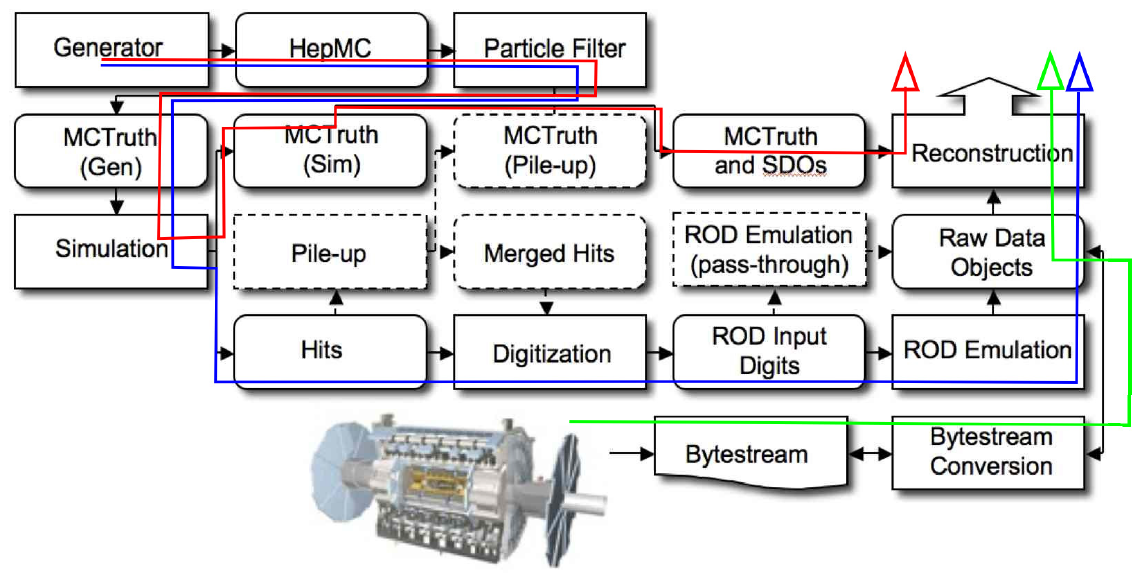
\includegraphics[width=\textwidth]{figures/EvtGen/atlassimul.png}
\captionsetup{width=0.85\textwidth} \caption{\small The flow of the ATLAS simulation software, from event generators (top left) through reconstruction (top right). The red path leads to particle level physics objects, the blue path to reconstructed level physics objects, while the green path shows the real data flow to physics objects. SDO stands for Simulated Data Object, ROD for Read Out Driver.}
\label{sec:evtgen:fig:ATLASsim}
\efig